
% Due thursday

\documentclass{article}

\usepackage[utf8]{inputenc}

\usepackage{amsmath, bm}
\usepackage{graphicx}
\usepackage{amssymb}
\usepackage{float}
\usepackage{caption}
\usepackage{subcaption}
\usepackage{hyperref}
\usepackage{tikz}
\usepackage{layout}

\usepackage[margin=1in]{geometry}
\usepackage{listings}
\usepackage{xcolor}
\usepackage{color, colortbl}
\usepackage{textgreek}
\usepackage{mathrsfs}
\usepackage{savetrees}


\setlength{\parskip}{\baselineskip}%
\setlength{\parindent}{0pt}%
\linespread{0.9}


\definecolor{codegreen}{rgb}{0,0.6,0}
\definecolor{codegray}{rgb}{0.5,0.5,0.5}
\definecolor{codepurple}{rgb}{0.58,0,0.82}
\definecolor{backcolour}{rgb}{0.95,0.95,0.92}

\lstdefinestyle{mystyle}{
    backgroundcolor=\color{backcolour},   
    commentstyle=\color{codegreen},
    keywordstyle=\color{magenta},
    numberstyle=\tiny\color{codegray},
    stringstyle=\color{codepurple},
    basicstyle=\ttfamily\footnotesize,
    breakatwhitespace=false,         
    breaklines=true,                 
    captionpos=b,                    
    keepspaces=true,                 
    numbers=left,                    
    numbersep=5pt,                  
    showspaces=false,                
    showstringspaces=false,
    showtabs=false,                  
    tabsize=2
}

\lstset{style=mystyle}



\begin{document}

\title{GA3: Heat Exchanger Final Report}
\author{lwp26}
\date{June 2024}
\maketitle 


\section{Introduction}

The development of heat exchanger design software is incomplete without real world performance evaluation.
This report covers the assembly, testing and final performance of the assembled design chosen by our software compared to those selected and built by other groups.

\section{Results}

\subsection{Group E Assembly}
A major design flaw appeared due to not considering a 1mm gap for the outer O ring between inner and outer shell lengths which forced use to increase tube length by 3mm.
Another small issue was that the compression cage did not allow the the nozzles to be 60 degrees apart, as specified by the drawings.
The diameter for small O rings and tubes was 0.36mm smaller than the value of 10.92 mm defined in the handout which was caused by instead defining the angle to be 45 degrees, which was not the case.
This issue made it harder to assemble the tubes, but also provided a better seal between cold and hot sections.
% nozzle problems
% baffle and end cap assembly problems
These issues immidiately highlight differences which were not accounted for in the uncertainty analysis in the previous performance report.

\begin{figure}[H]
    \centering
    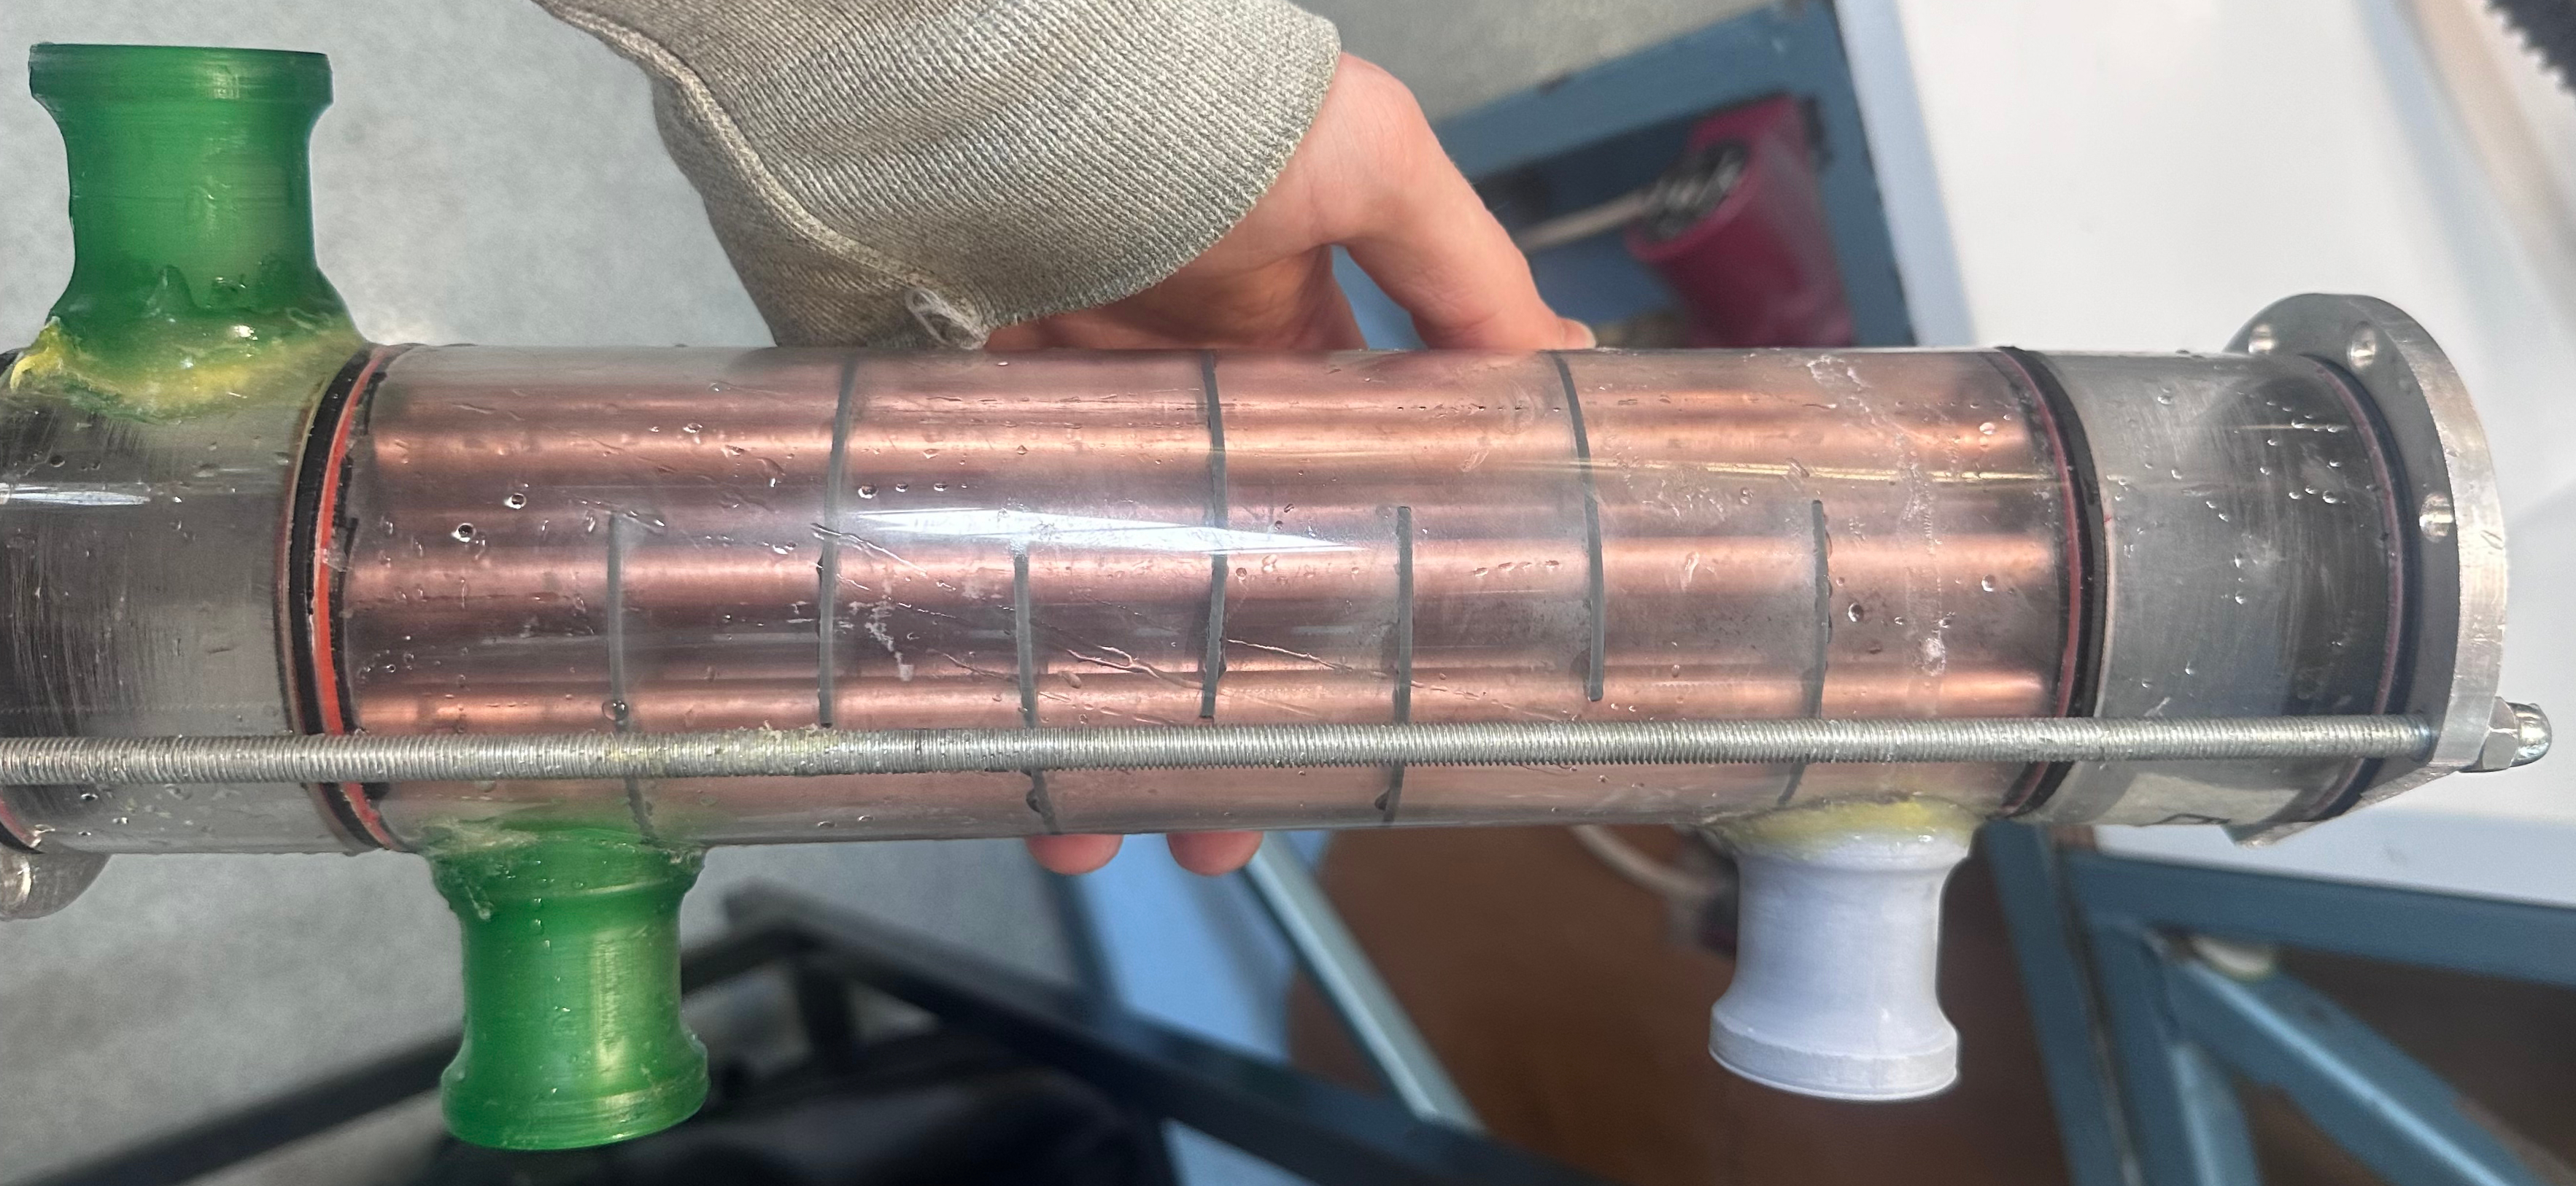
\includegraphics[width=0.5\textwidth]{final_tested.jpg}
    \caption{Final tested heat exchanger}
    \label{fig:heat_exchanger}
\end{figure}

\section{Results}

\iffalse
\begin{figure}[H]
    \centering
    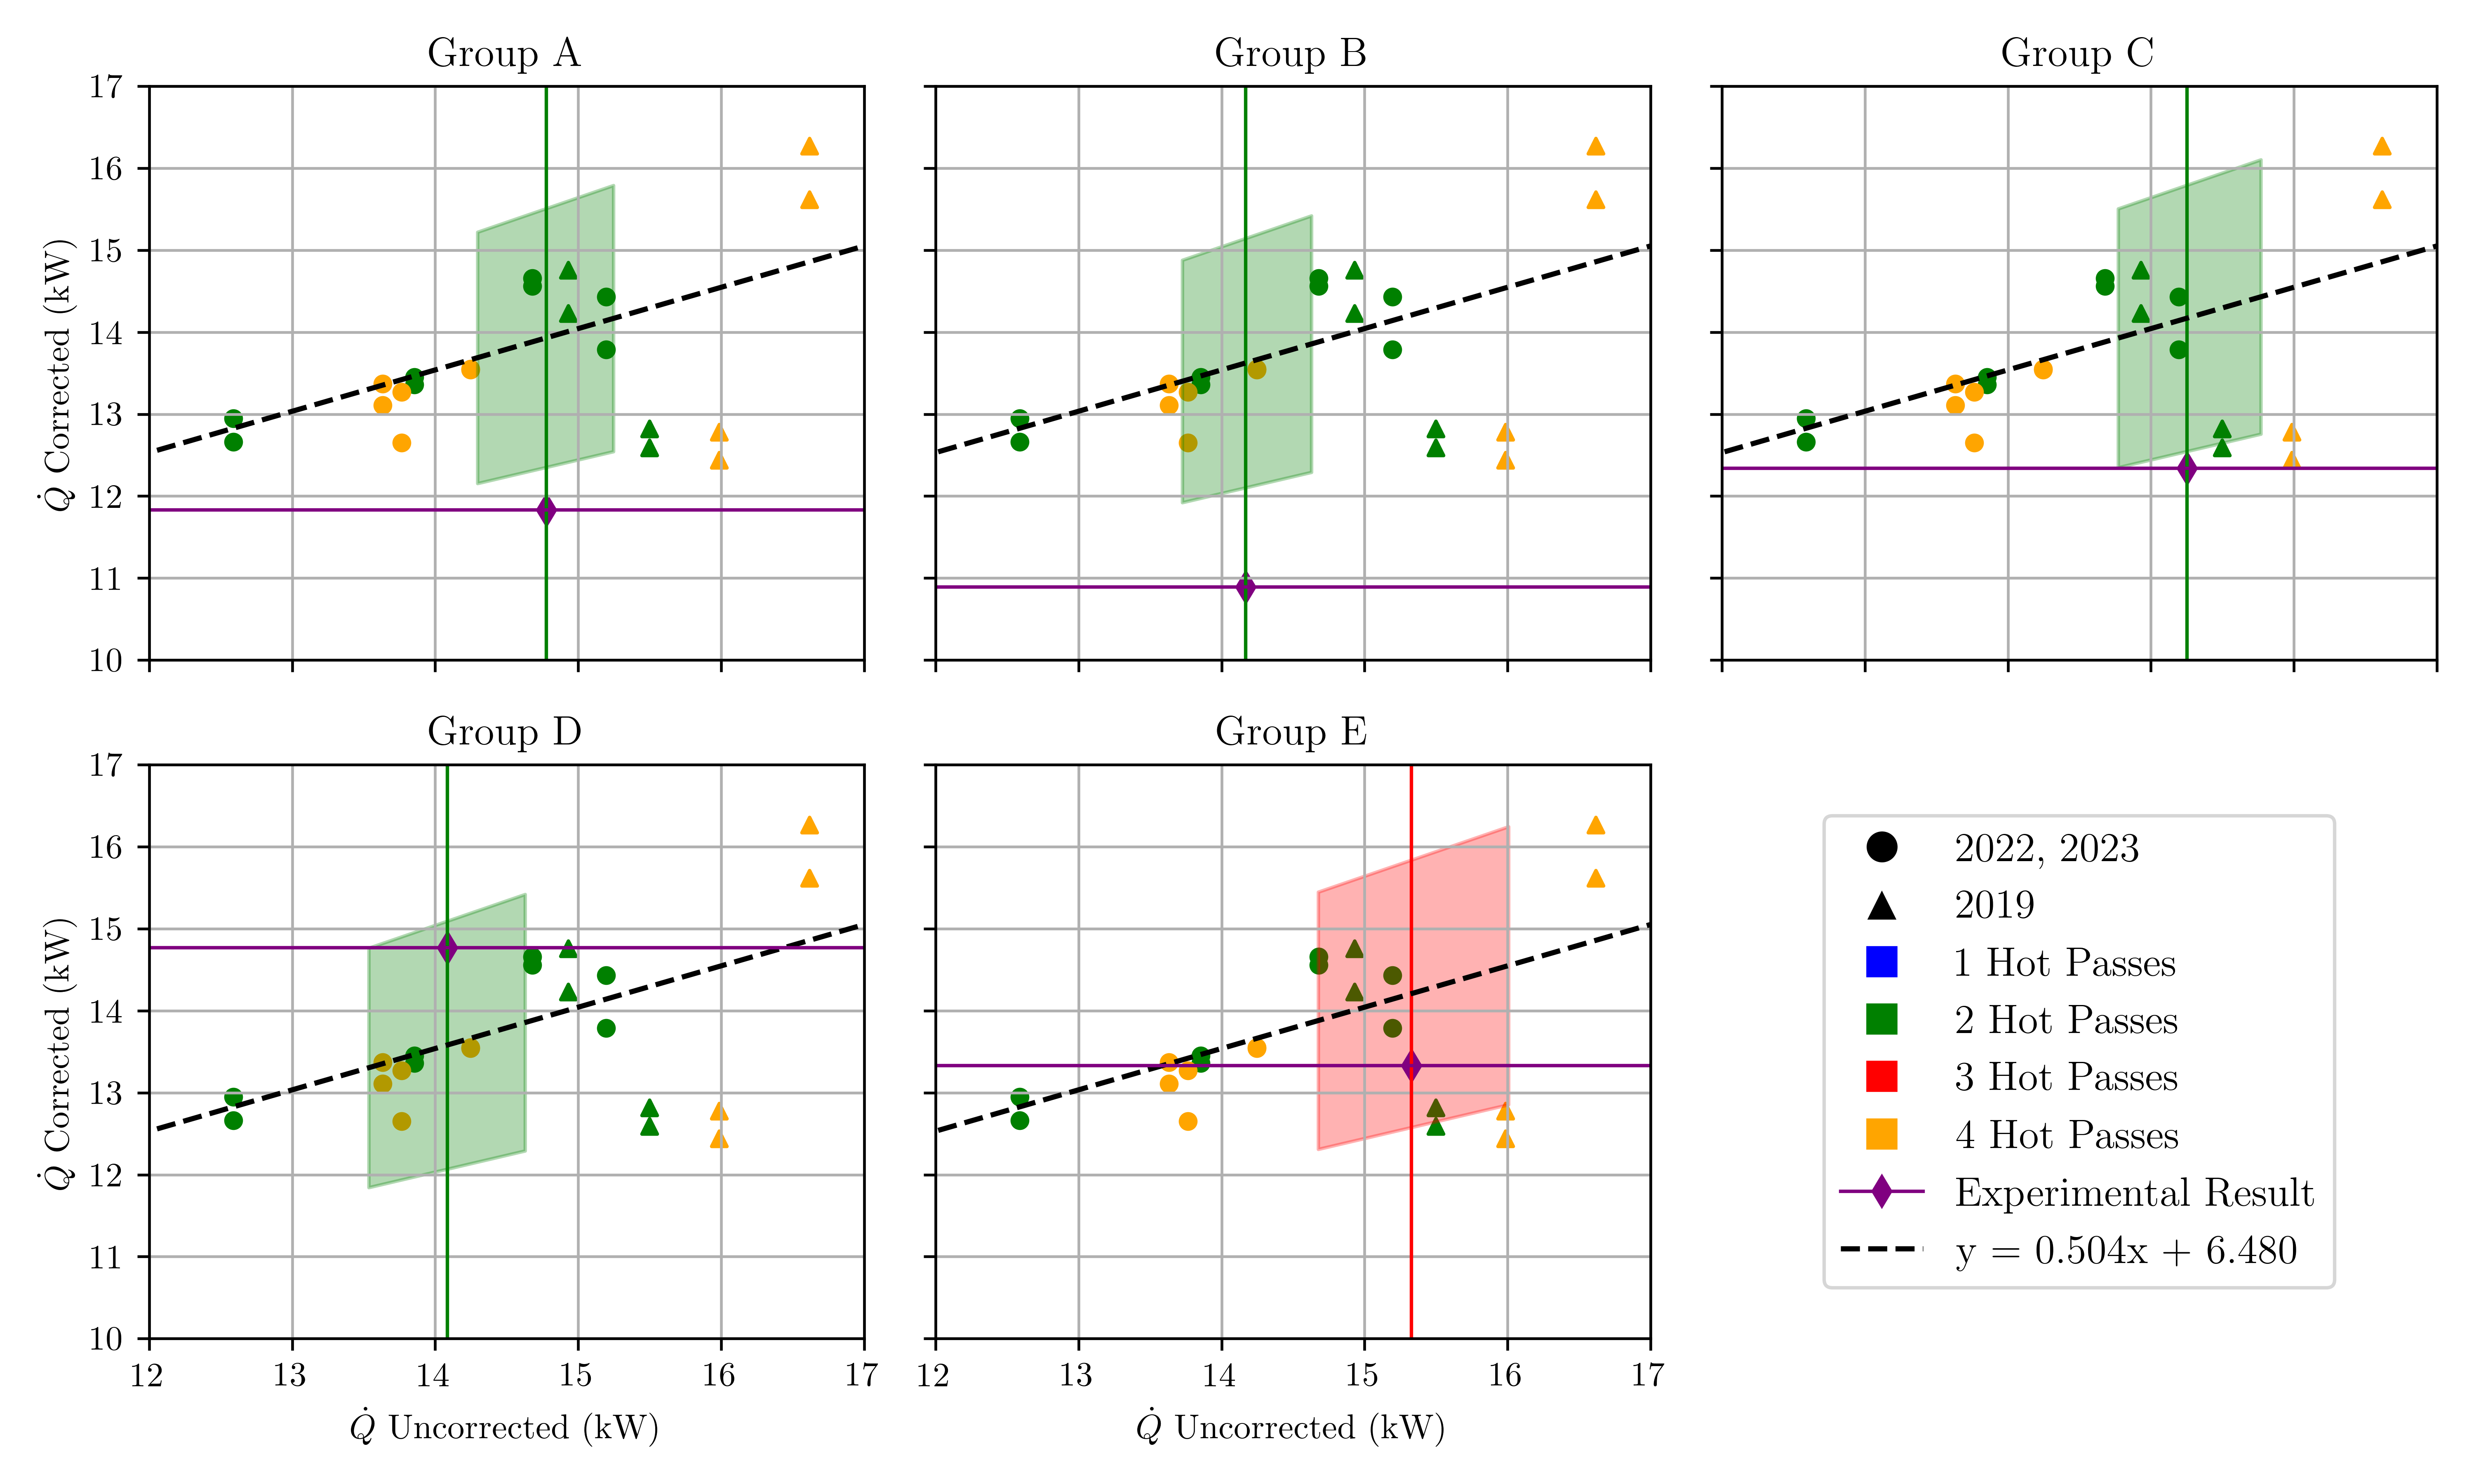
\includegraphics[width=0.9\textwidth]{Qdot_result_bands.png}
    \caption{Qdot results}
    \label{fig:Qdot_results}
\end{figure}
\fi

\begin{figure}[H]
    \centering
    \begin{subfigure}{0.8\textwidth}
        \centering
        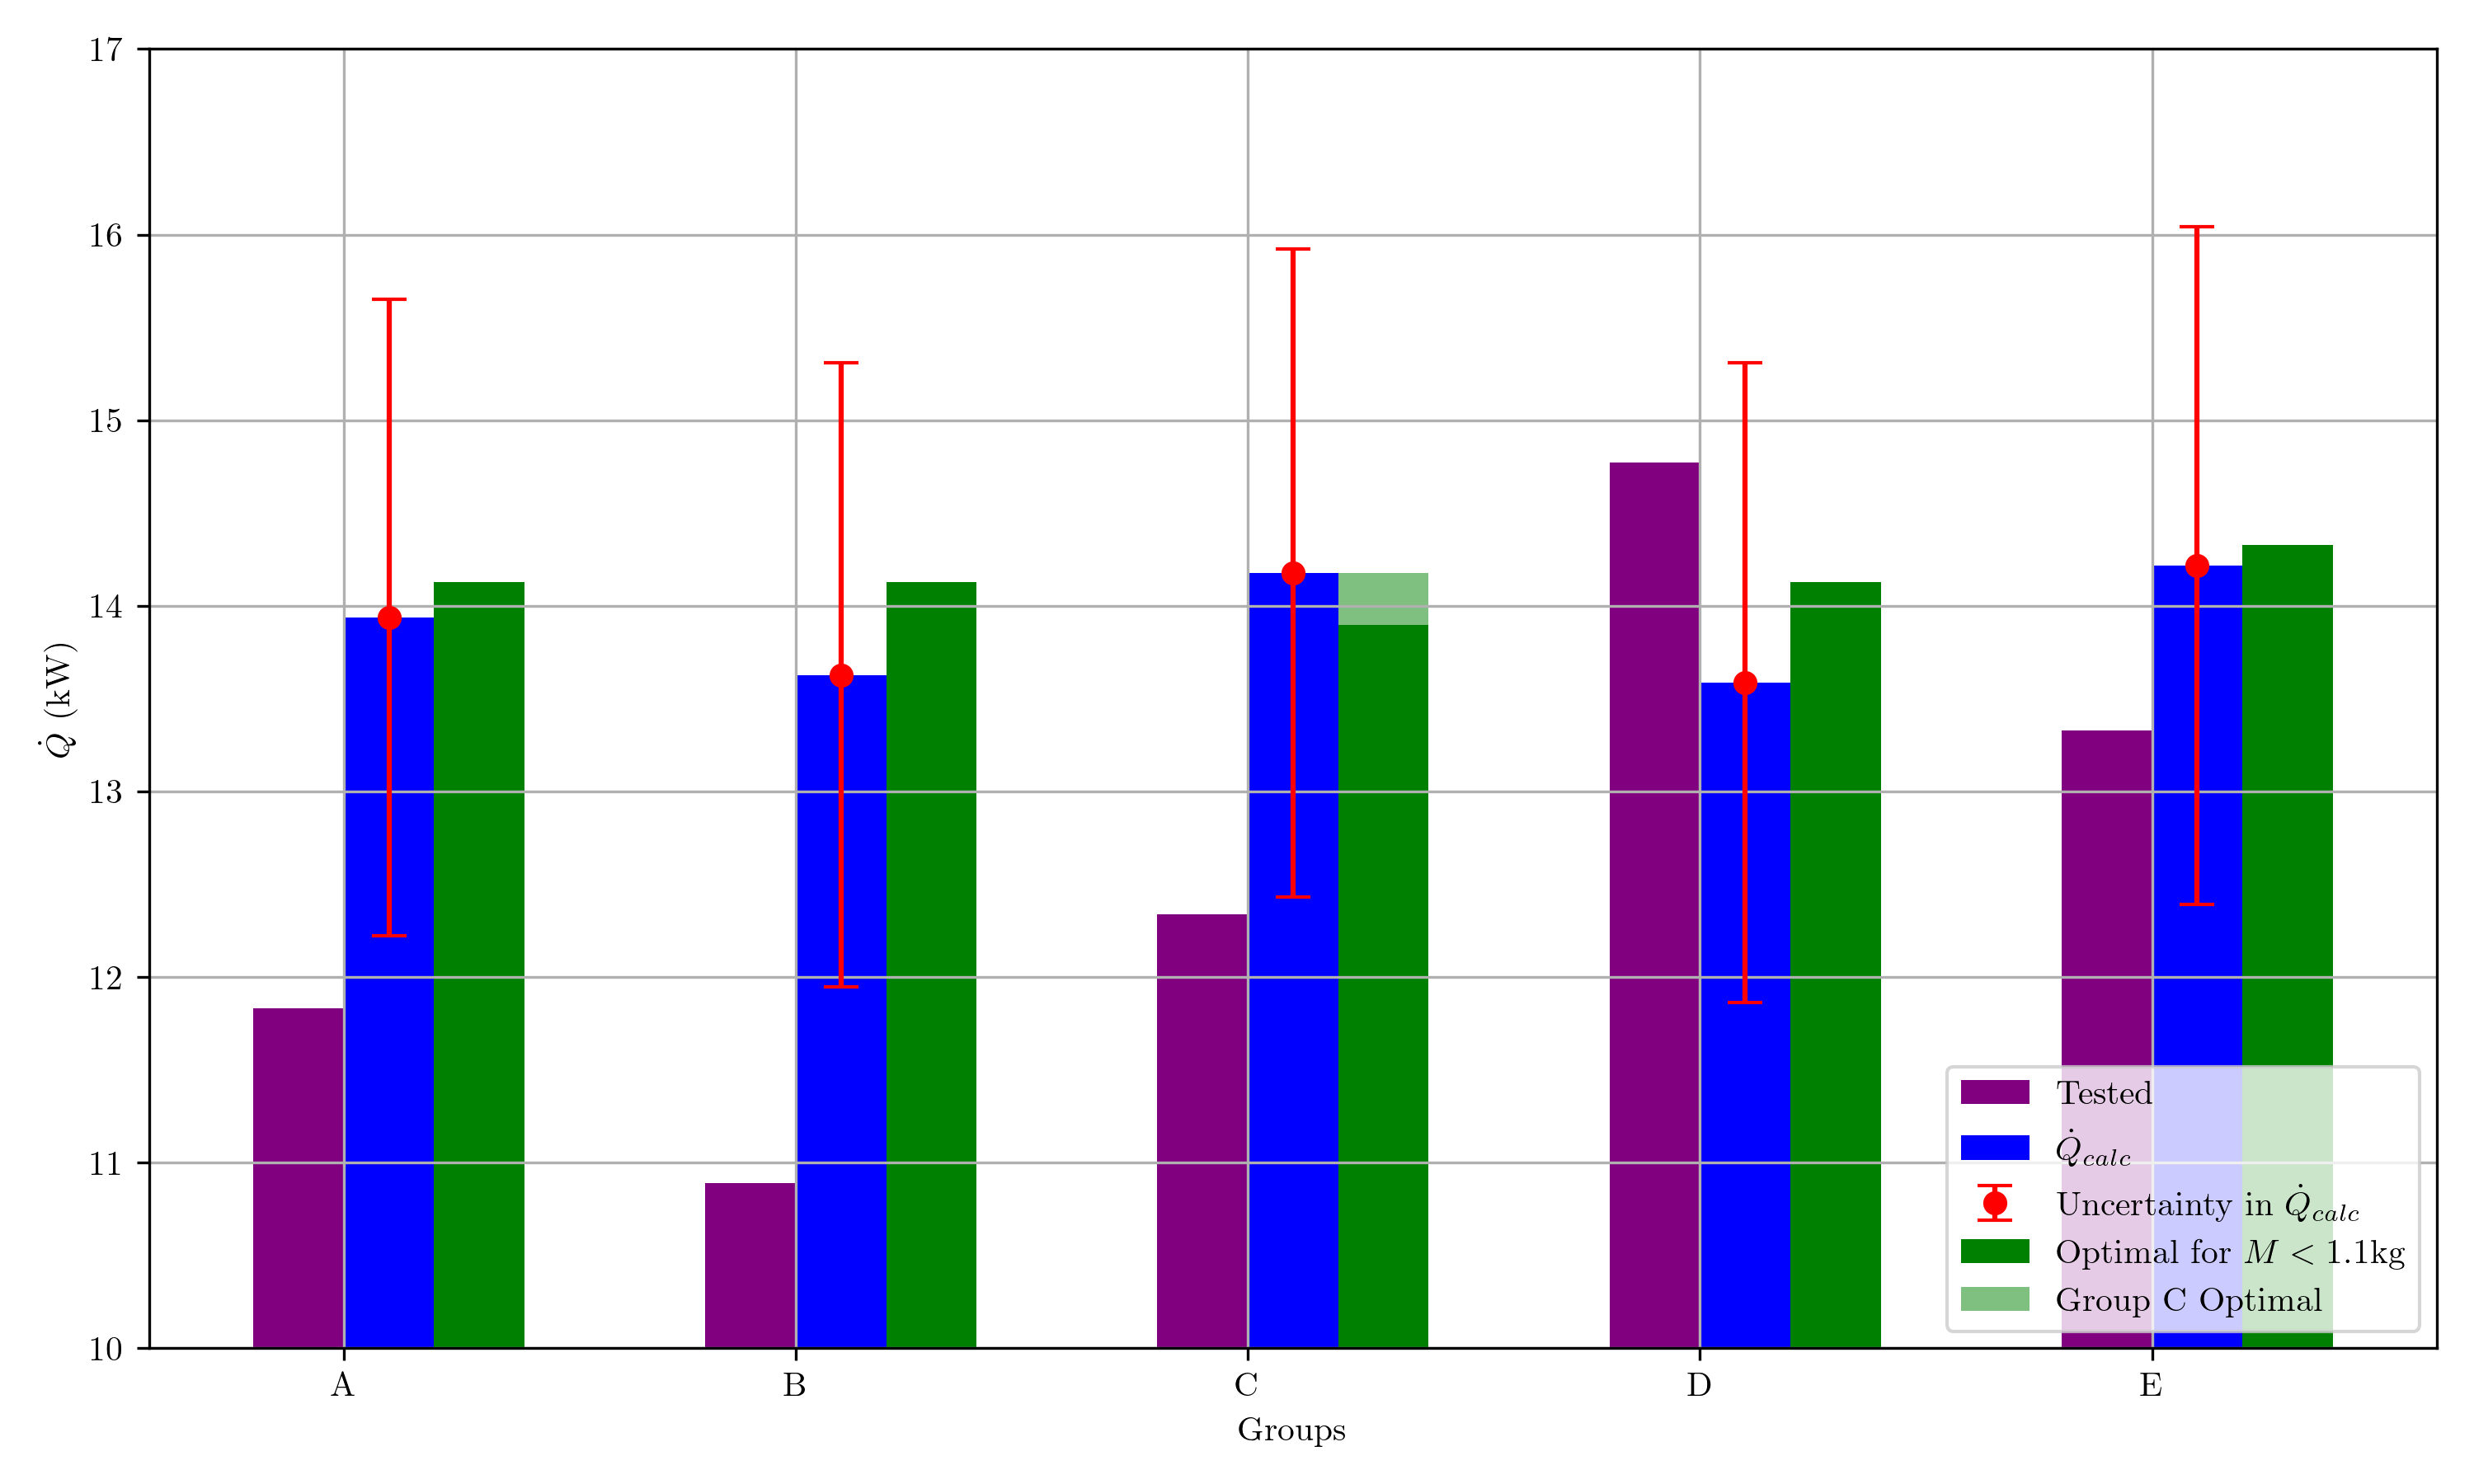
\includegraphics[width=0.8\textwidth]{2024_results.png}
        \captionof{figure}{$\dot{Q}$ results}
        \label{fig:Qdot_results} 
    \end{subfigure}
    \begin{subfigure}{0.9\textwidth}
        \centering
        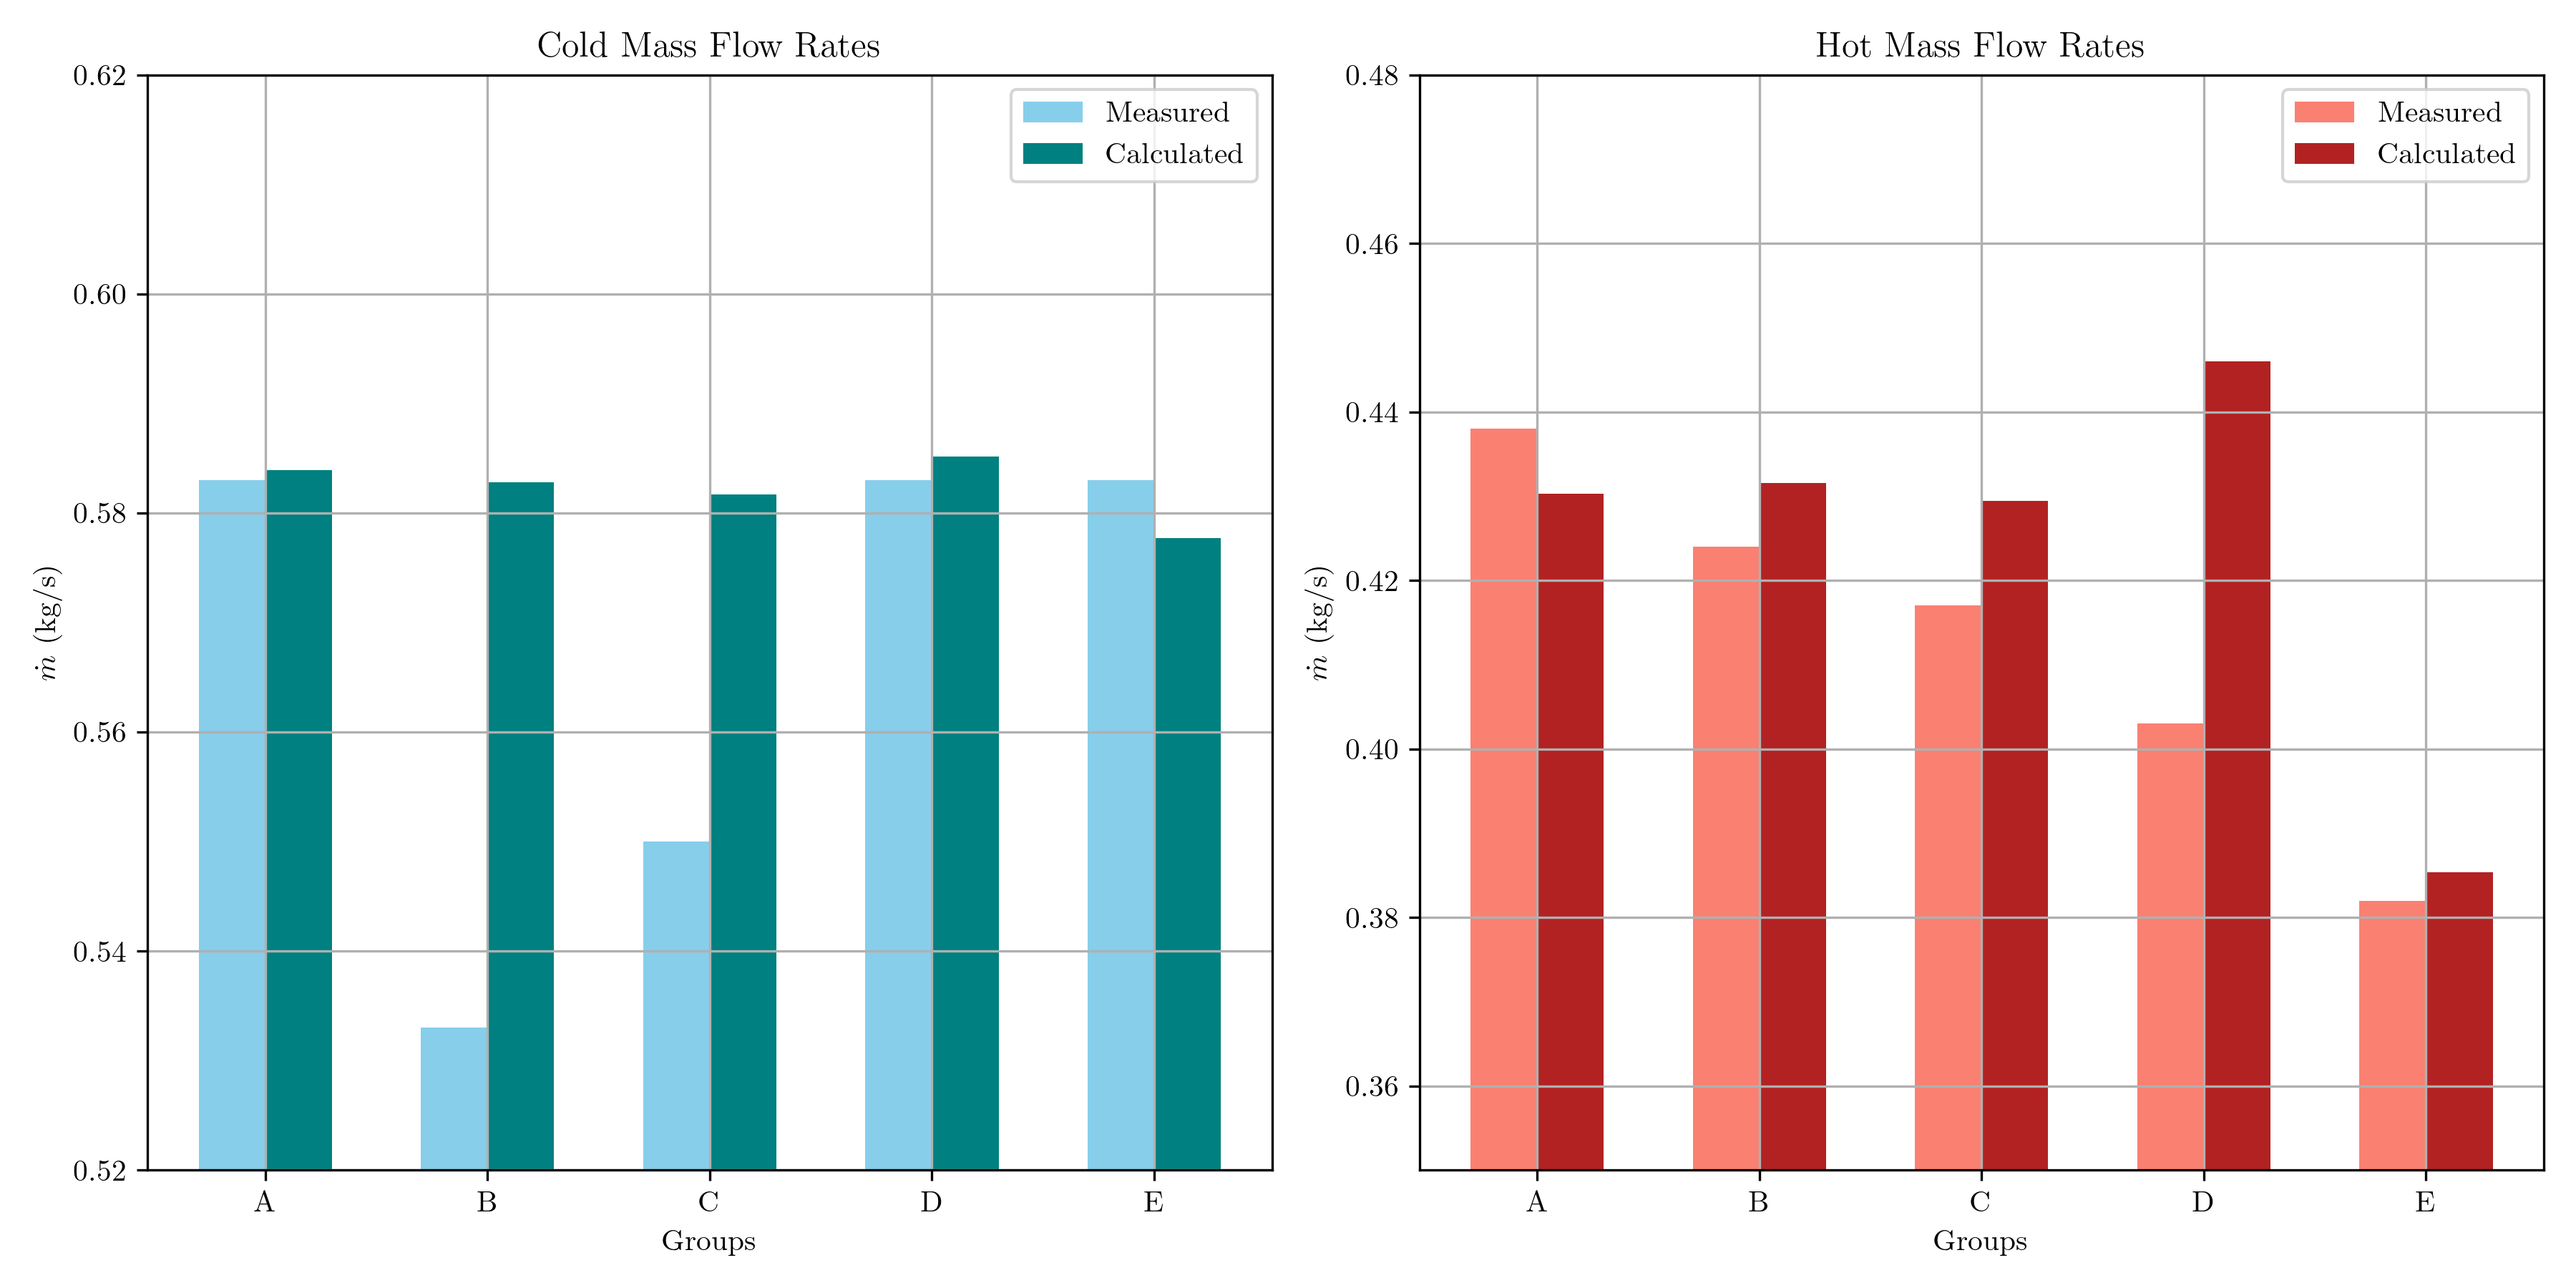
\includegraphics[width=0.99\textwidth]{2024_mass_flow_rates.png}
        \captionof{figure}{Mass flow rates of hot and cold sides for each group}
        \label{fig:mdot_results}
    \end{subfigure}
    \caption{Results}
\end{figure}

Figure \ref{fig:Qdot_results} shows the experimental results for the heat exchanger performance of each group.
Group D's heat exchanger performed the best at 14.77 kW, exceeding our calculated value by 8.7\%, but within the uncertainty band of 12.69\%.
Our group E heat exchanger had the second best performance 9.7\% below that of Group D, and 6.2\% below our calculated value.
The remaining groups ranked C, A and then B at 16.5\%, 19.9\% and 26.3\% below group D, which is the same order predicted by our software.
Figure \ref{fig:Qdot_results} also shows that these last 3 groups are outside of the uncertainty bands with experimental values being
-13.0\%, -15.1\% and -20.1\% below the respective calculated values.
% explain discrepency in B and C using poorly calculated cold mass flow rates due to kerns method again
% A is hard to explain as mass flow rates agree with calculations they did leak though
% comment on group C hot flow being lower than expected due to underestimating pressure drop of their special manifold


\newpage

% more detailed fouling, comparison with bell delaware method
% additional constraints and design considerations for variety of applications:
% - optimal performance at a range of operating conditions
% - robustness to fouling and ease of maintenance
% - cost of materials and manufacturing at scale
% - ease of assembly and disassembly
% software improvements

\section{Future Work}

\begin{itemize}
    \item Implementing and comparing the Bell-Delaware method with Kerns method for more accuate shell side pressure drop calculations.
    \item Additional constraints and design considerations could be incorporated into the software to cater to a variety of applications:
    \begin{itemize}
        \item Optimizing the heat exchanger performance over a range of inlet temperatures or compressor characterisitcs.
        \item Enhancing the design's robustness to fouling and ease of maintenance to minimize costs and extend the heat exchanger's lifespan.
        \item Considering the cost of materials and manufacturing at scale of the designed heat exchangers.
        \item Improving the ease of assembly and disassembly to facilitate installation, maintenance, and replacement of components.
    \end{itemize}

    \item The heat exchanger design software can be further improved by:
    \begin{itemize}
        \item Refining the user interface and user experience to make it more intuitive and user-friendly.
        \item Exporting optimised designs to a design table for rapid prototyping of 3D models.
    \end{itemize}
\end{itemize}


\section{Recommendations}
% hard section to write
% a 3-1 configuration is recommended for this application
% despite textbooks stating that an odd number of hot passes 
% with more counterflow passes than coflow passes may result in structural and thermal problems

An odd number of hot passes, with more counterflow passes than coflow passes, has a slightly better effectiveness
than an even number of hot passes with an equal number of coflow and counterflow.
This comes at a cost of increased pressure drop compared to a smaller number of even hot passes.
Textbooks (meant for larger heat exchangers) state these uncommon designs may result in structural and thermal problems \cite{},
However for this application of compact heat exchangers, the increased effectiveness was found to be worth the tradeoff.
% However, this is an uncommon design and may result in structural and thermal problems in manufacturing and design.

% baffle count
% tube count
% tube position ?

\section{Conclusion}

\begin{thebibliography}{9}

%Endres, SC, Sandrock, C, Focke, WW (2018) “A simplicial homology algorithm for lipschitz optimisation”, Journal of Global Optimization.

\iffalse
    \bibitem{handout}
    J. V. Taylor and J. C. Massey
    \emph{GA3 Heat Exchanger Handout}
    University of Cambridge,
    2024.
\fi

    \bibitem{HeatTransfer}
    Holman J. P.
    \emph{Heat Transfer. 10th ed.}
    McGraw-Hill,
    2010.

    \bibitem{HE_design}
    Sadik Kakac, Hongtan Liu, Anchasa Pramuanjaroenkij,
    \emph{Heat Exchangers: Selection, Rating, and Thermal Design, Third Edition}
    CRC Press,
    2012.


\end{thebibliography}

\end{document}